% \documentclass{report}

% \usepackage{fancyhdr}
\usepackage{fourier-orns}
\usepackage{hyperref}%% To refrence links / jumps
\usepackage{chngcntr} %% For some extra counters numberings
\usepackage[a4paper, right = 0.5in, left = 0.5in,top = 1in , bottom = 1in]{geometry}
\usepackage{etoolbox} %% Provides like a language for advanced customization
\usepackage{datetime} %% For dates of course
\usepackage{lastpage} %% provides pages numbers
\usepackage[sc]{titlesec} %% modify titles
\usepackage{enumerate}
\usepackage{cancel}
\usepackage{tikzsymbols}
\usepackage[dvipsnames]{xcolor}
\usepackage{import}
\usepackage{pdfpages} %% include other pdfs
\usepackage{transparent} %% Transparency
\usepackage{xcolor}  %% Colors
\usepackage[many]{tcolorbox}
\usepackage[framemethod=TikZ]{mdframed}
\usepackage{amsmath,amsfonts,amsthm,amssymb,mathtools}
\usepackage{tikz}
\usepackage{bookmark}
\usepackage{graphicx}
\usepackage{mathpazo}

\usepackage{fontawesome5}

\linespread{1.5}


\titleformat{\chapter}[display]   
{\fontfamily{ppl}\selectfont\huge\color{YellowOrange!80!orange}} % Font style and size 
{\raggedleft\color{purple}\fontsize{70}{0pt}\selectfont\thechapter}   
{-1.5cm}    			                          % Space between the chapter number and title
{
	\begin{tikzpicture}[overlay]
		\node[anchor = west,yshift = 0.2cm,xshift = -1cm] {\fontsize{90}{20} $\int_{}^{} $};
		\node[yshift = 4cm, xshift = 17cm]   {\includegraphics[width = 4cm]{preview0}};
	\end{tikzpicture}
\hspace{1cm}\Huge\raggedright\MakeUppercase}

\titleformat{\section}[block]
{
\fontfamily{ppl}\selectfont\huge\color{YellowOrange!80!orange}
}
{
\color{purple}\fontsize{20}{0pt}\selectfont\thesection 
}
{0cm}
{
	\begin{tikzpicture}[overlay]
		\node[anchor = west,yshift = 0.2cm,xshift = -0.4cm, circle = 1pt] {};
	\end{tikzpicture}
}

\titlespacing*{\section}{0pt}{0.7cm}{1.5cm}


\newcommand{\divider}
{
	\begin{center}
	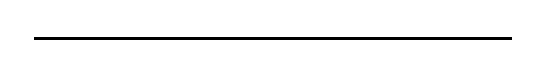
\begin{tikzpicture}
		\draw[thick, black] (0.25*\textwidth, 0) -- (0.75*\textwidth, 0);
		\node[rotate = 360 - 90, xshift = -0.6pt, yshift = 1pt] at (0.25*\textwidth,0){\decotwo};
		\node[rotate = 90, xshift = -0.6pt, yshift = 1pt] at (0.75*\textwidth,0){\decotwo};
	\end{tikzpicture}
	\end{center}
}

\pagestyle{fancy}

\newcommand{\lecday}[1][]
{
    \def\datee{#1}
    \fancyhead[L]{\datee}
}



\newcommand{\signature}
{
	\begin{tikzpicture}[remember picture,overlay]
		\node[fill = YellowOrange!20!white] at ([yshift = 1cm, xshift = -3cm]current page.south east) {\fontsize{10pt}{0pt}{\itshape Kara.$\mathcal{A}$}};
	\end{tikzpicture}
}

\AddToHook{shipout/background}{
  \begin{tikzpicture}[remember picture, overlay]
	  \node[] at ([yshift = 1.5cm,xshift = \textwidth /2 + 0.9cm]current page.south west) {\includegraphics[width = 0.5cm]{preview3}};
	  \node[] at ([yshift = 1.5cm,xshift = - \textwidth /2 - 0.9cm]current page.south east) {\includegraphics[width = 0.5cm]{preview4}};
  \end{tikzpicture}
}



\newtcolorbox[auto counter, number within = section]{remark}[1][]
{
       		title = Remark #1,
		enhanced,
		boxrule = 0pt,
		colback = white,
		breakable,
		arc = 4pt,
		colbacktitle = cyan,
		colback = cyan!5!white,
		segmentation style =
		{
			solid,cyan,thick,
		},
		attach boxed title to top left =
		{
			xshift = 0cm,
		},
		boxed title style =
		{
			boxrule = 0pt,
			sharp corners,
			drop fuzzy shadow = {cyan},
		},
		drop fuzzy shadow = {cyan!80!black},
}

\newtcolorbox[auto counter, number within = section]{theorem}[1][]
{                                      
		title = Theorem \thetcbcounter : #1,
		enhanced, 
		boxrule = 0pt,
		colback = white,
		breakable,
		arc = 4pt,
		colbacktitle = purple,
		colback = purple!5!white,
		segmentation style = 
		{
			solid, purple,thick,
		},
		attach boxed title to top left = 
		{
			xshift = 0cm, 
		},
		boxed title style = 
		{
			boxrule = 0pt,
			sharp corners,
			drop fuzzy shadow = {purple},
		},
		drop fuzzy shadow = {purple!80!black},
}

\newtcolorbox[auto counter, number within = section]{definition}[1][]
{                                      
		title = Definition \thetcbcounter : #1,
		enhanced, 
		boxrule = 0pt,
		colback = white,
		arc = 4pt,
		breakable,
		colbacktitle = YellowOrange!80!black,
		segmentation style = 
		{
			solid, YellowOrange,thick,
		},
		attach boxed title to top left = 
		{
			xshift = 0cm, 
		},
		colback = YellowOrange!5!white,
		boxed title style = 
		{
			boxrule = 0pt,
			sharp corners,
			drop fuzzy shadow = {YellowOrange!80!orange},
		},
		drop fuzzy shadow = {YellowOrange!80!black},
}

\newtcolorbox[auto counter, number within = section]{corollary}[1][]
{                                      
		title = corollary \thetcbcounter : #1,
		enhanced, 
		boxrule = 0pt,
		colback = white,
		arc = 4pt,
		breakable,
		colbacktitle = YellowOrange!80!black,
		segmentation style = 
		{
			solid, YellowOrange,thick,
		},
		attach boxed title to top left = 
		{
			xshift = 0cm, 
		},
		colback = YellowOrange!5!white,
		boxed title style = 
		{
			boxrule = 0pt,
			sharp corners,
			drop fuzzy shadow = {YellowOrange!80!orange},
		},
		drop fuzzy shadow = {YellowOrange!80!black},
}


\newtcolorbox{example}[1][]
{                                      
		title = Example,
		enhanced, 
		boxrule = 0pt,
		colback = white,
		arc = 4pt,
		segmentation style = 
		{
			solid, SpringGreen,thick,
		},
		breakable,
		colback = SpringGreen!5!white,
		colbacktitle = SpringGreen!80!black,
		attach boxed title to top left = 
		{
			xshift = 0cm, 
		},
		boxed title style = 
		{
			boxrule = 0pt,
			sharp corners,
			drop fuzzy shadow = {SpringGreen!80!orange},
		},
		drop fuzzy shadow = {SpringGreen!80!black},
}


\newcommand{\integral}[4]{\int\limits_{#1}^{#2} #4 d#3}
\newcommand{\limit}[3]{\lim\limits_{#1 \rightarrow #2} #3}
\newcommand{\strone}[2]{\left[ \begin{gathered}#1\\ #2\end{gathered} \right] }
\newcommand{\strtwo}[2]{\left\{ \begin{gathered}#1\\ #2\end{gathered} \right\} }
\newcommand{\strthree}[2]{\left\lfloor \begin{gathered}#1\\ #2\end{gathered} \right\rfloor }


\newcommand{\startbf}[1]{\text{\bfseries{#1}}}
\newcommand{\sett}[1]{\left\{ #1 \right\}}
\newcommand{\thesis}[1]{\left( #1 \right)}
\newcommand{\brkt}[1]{\left[ #1 \right]}
\newcommand{\floor}[1]{\left\lfloor #1 \right\rfloor}


\DeclareMathOperator{\img}{im} % Image
\DeclareMathOperator{\Img}{Im} % Image
\DeclareMathOperator{\coker}{coker} % Cokernel
\DeclareMathOperator{\Coker}{Coker} % Cokernel
\DeclareMathOperator{\Ker}{Ker} % Kernel
\DeclareMathOperator{\rank}{rank}
\DeclareMathOperator{\Spec}{Spec} % spectrum
\DeclareMathOperator{\Tr}{Tr} % trace
\DeclareMathOperator{\pr}{pr} % projection
\DeclareMathOperator{\ext}{ext} % extension
\DeclareMathOperator{\pred}{pred} % predecessor
\DeclareMathOperator{\dom}{dom} % domain
\DeclareMathOperator{\ran}{ran} % range
\DeclareMathOperator{\Hom}{Hom} % homomorphism
\DeclareMathOperator{\Mor}{Mor} % morphisms
\DeclareMathOperator{\End}{End} % endomorphism


\newcommand{\lm}{\ensuremath{\lambda}}
\newcommand{\eps}{\ensuremath{\epsilon}}
\newcommand{\veps}{\ensuremath{\varepsilon}}
\newcommand{\al}{\ensuremath{\alpha}}
\newcommand{\bb}{\ensuremath{\beta}}
\newcommand{\cc}{\ensuremath{\gamma}}
\newcommand{\dd}{\ensuremath{\delta}}
\newcommand{\DD}{\ensuremath{\Delta}}
\newcommand{\ff}{\ensuremath{\phi}}
\newcommand{\FF}{\ensuremath{\varphi}}

\newcommand{\RR}{\mathbb{R}}
\newcommand{\RO}{\mathcal{R}}
\newcommand{\EE}{\mathbb{E}}
\newcommand{\CC}{\mathbb{C}}
\newcommand{\RW}{\mathbb{R}^2}
\newcommand{\RT}{\mathbb{R}^3}
\newcommand{\RN}{\mathbb{R}^n}
\newcommand{\DS}{\mathcal{D}}

\newcommand{\KK}{\mathbb{K}}
\newcommand{\KW}{\mathbb{K}^2}
\newcommand{\KT}{\mathbb{K}^3}
\newcommand{\KN}{\mathbb{K}^n}

\newcommand{\NN}{\mathbb{N}}

\newcommand{\PS}{\mathcal{P}}
\newcommand{\AS}{\mathcal{E}}
\newcommand{\FS}{\mathcal{F}}
\newcommand{\LS}{\mathcal{L}}
\newcommand{\MS}{\mathcal{M}}


















\lecday[2025-02-05]
% \begin{document}
\chapter{The concept of a norm on a real or complex vector space}	
	For all what follows $\KK$ denotes one of the two feild $\RR$ or $\CC$ and $\left| . \right|$ denotes the absolute value
	if $\KK=\RR $ and the modulus if $\KK=\CC $.

	\section{Norm on a \texorpdfstring{$\KK$}{K}-vector space}
	\begin{definition}[Norm]
		Let $E$ be a $\KK$-vector space, we call a norm on $E$ every map $ \| . \|  : E \longrightarrow [0, \infty) $
		satisfiying the following properties:
		\begin{enumerate}[(i)]
			\item $\forall x \in E: \quad \| x \| = 0 \implies x=0_{E}$
			\item $\forall x \in E, \forall \lm \in \KK: \quad \| \lm x \| = \left| \lm \right| \| x \|  $               
			\item $\forall x,y \in E: \quad \| x + y \| \leq  \| x \| \| y \| $
		\end{enumerate}
	
	\end{definition}
	\begin{remark}[]
		\begin{itemize}
			\item A $\KK$-vector space E equipped with a norm $\| . \| $ is called \textbf{a normed vector spcae}
				(abbreviated to N.V.S), it is written $(E,\| . \| ) $ or simply $E$ if there is no ambiguity
				about the norm $\| . \|$
			\item   The equivallence "$\iff$" in (i) can be replaced by the implication "$\implies$" because the implication
				\\ $(x = 0_{E} \implies \| x \| = 0) $ can be obtained from property (ii) by taking $\lm = 0$
			\item Inequality in (iii) is called \textbf{"The Triangle Inequlity"} or \textbf{"The Convex Inequality"},
				it is equivalent to say that the norm $\| . \|$ is a convex function on $E$, that is:
				\[
					\forall t \in (0,1) ,\forall x,y \in E: \quad \| tx + (1-t)y  \| \leq t\| x \| + (1-t)\| y \|  
				\]
				Indeed, we have:
				\begin{align*}
					\| tx + (1-t)y  \| & \leq \|t x \| + \|(1-t) y \| \\
							   & \leq \left| t \right| \| x \| + \left| 1-t \right|\| y \|
							   & \leq t \| x \| + (1-t) \| y \|  	
				\end{align*}
				$t = \frac{1}{2}$: we get it
			\item if $E$ is a $\KK$-vector space and $ \| . \|  : E \longrightarrow [0, \infty) $ satisfies just properties
				(i) and (ii) then $\| . \| $ is called a \textbf{seminorm on $E$} (so seminorm could assing 0 to non-zero
				vectors), the pair $(E,\| . \| )$ is then called a \textbf{Seminormed Vector Space}.
		\end{itemize}
	\end{remark}           

	\section{Metric Associated to a Norm}
	\begin{definition}[]
		Let $(E, \| . \| )$ be a N.V.S, Define:
		\[
		\begin{array}{cccc}
			d : &  E^{2}  & \longrightarrow & [0, \infty) \\
		
		           &  (x,y)   & \longmapsto     & d(x,y) = \| x-y \|   \\ 
		\end{array}
		\]
		we can easily verify that $d$ is a metric on $E$, and it is called \textbf{The Metric Associated To The Norm $\| . \| $}
		or \textbf{The Generated Metric By The Norm}
	\end{definition}
	\begin{remark}
		\begin{itemize}
		\item Thanks to the concept of the metric generated by a norm, a N.V.S is seen as a particular metric space, which is a
			particular topological space.
		\item The definition of the open ball, a closed ball, a sphere, an open set, a closed set, a neighborhood,the interior 
			of a set, limit, the closure of a set,etc... in a N.V.S are those related to the metric generated by the norm.

		\item Every metric $d$ generated by a norm (in a given N.V.S $E$) is invarient by translation, that is:
			\[
				\forall x,y,z \in E: \quad d(x+z,y+z) = d(x,y)  
			\]
		\item There exist natural metric that are not generated by any norm (like discrect distance).
		\end{itemize}
	\end{remark}

	\section{Examples of some concepts on a N.V.S derived from its metric structure}
	\begin{enumerate}                                                                                            
	\item Let $(E,\| . \| ) $ be a N.V.S, $(x_{n})_{n \in \NN}$ be a sequence of $E$, and $x$ be a vector of $E$.
		\begin{itemize}
			\item We say that $(x_{n})_{n \in \NN}$ converges to $x$ if we have $\lim_{n \to \infty} \| x_{n} -x \| =0$,
				equivallently:
				\[
					\forall \veps > 0, ~\exists N \in \NN \quad \text{s.t } \quad  \forall n \in \NN \quad 
					(n>N \implies \| x_{n} -x \| )  
				\]
				in this case we write $\lim_{n \to \infty} x_{n}  = x$ or $x_{n} \rightarrow x$ on $n \rightarrow \infty$
			\item We say that $(x_{n})_{n \in \NN}$ is a cuachy sequence if we have 
				$\lim_{p,q \to \infty} \| x_{p} - x_{q}\| = 0$, equivalantly:
				\[
					\forall \veps > 0, ~\exists N \in \NN: ~\forall p,q \in \NN \quad 
					(p>q>N \implies \| x_{p} - x_{q}\| < \veps  ) 
				\]	
		\end{itemize}
	\item Let $(E,\| . \|_{E} )$ and $(F,\| . \|_{F} )$ be two N.V.S over the same field $\KK$, 
		$ f : E \longrightarrow F $ be a map from $E$ to $F$, Let $x_0 \in  E$ and $y_0 \in F$,
		\begin{itemize}
			\item We say that $f(x)$ tends to $y_{0}$ when x tends to $x_0$ (and we write $\lim_{x \to x_0} f(x) = y_0$ or
				$f(x) \rightarrow y_0$ as $x \rightarrow x_0$  )
				\[
				\begin{cases}
					\forall \veps >0, ~\exists \eta >0, \quad \text{s.t} \quad \forall x \in E: \\
					\| x-x_0 \| _{E} < \eta \implies \| f(x) - y_0  \| _{F} < \veps 
				\end{cases}
				\]
			\item We say that $f$ is continious at $x_0$ if we have:
				\[
					\lim_{x \to x_0} f(x) = f(x_0)  
				\]
			that is,
			\[
				\begin{cases}
					\forall \veps >0, ~\exists \eta >0, \quad \text{s.t} \quad \forall x \in E: \\
					\| x-x_0 \| _{E} < \eta \implies \| f(x) - f(x_0)  \| _{F} < \veps 
				\end{cases}
			\]
			\item We say that $f$ is continious on E if it is continious at all vector $x$ of $E$.
			\item We say that $f$ is uniformally continious on E if we have $\forall \veps >0, \exists \eta >0$ such that
				$\forall x,y \in E$:
				\[
				\| x-y \| _{E} < \eta \implies \| f(x) - f(y)  \| _{F} < \veps 
				\]
			\item Let $M>0$, wz say that $f$ is M-lipchitz if we have:
				\[
					\forall x,y \in E: \quad \| f(x)  - f(y) \|_{F} \leq M\| x-y \| _{E}
				\]
			\item We say that $f$ is a contraction if it is M-lipchitz for some constant $M \in (0,1)$, Note that/
				\[
				\text{Lipchitz Continious} \implies \text{Uniformally Continious} \implies \text{Continious}   
				\]
		\end{itemize}
	\end{enumerate}

	\section{Equivalent and Topologically Equivalent Norms}
	\begin{definition}[]
		Let $E$ be a $\KK$-vector space and $N_1$ and $N_2$ two norms on $E$:
		\begin{itemize}
			\item We say that $N_1$ and $N_2$ are topologically equivallent if their associated ,etrics are topologically 
				equivalent, that is they induce the same topology on $E$.
			\item We say that $N1$ and $N2$  are equivalent if their associated metrics are equivalent, that is their exist
				$ \alpha,\beta>0$ such that:
				\[
					\alpha N_1 \leq N_2 \leq \beta N_1 \quad  \quad 
					(\text{i.e} \quad \forall x \in  E: \quad \alpha N_1(x)  \leq N_2(x)  \leq \beta N_1(x)  ) 
				\]
		\end{itemize}
	\end{definition}
	\begin{remark}[]
		\begin{itemize}
			\item   It is known that two equivalent metrics (on a given non-empty set) are topologically equivalent 
				but the inverse is generally false.
			\item  Note that in a $\KK$-vector space, the two concepts "equivalent norms" and "topologically
				equivalent norms" coincide   
			\item  We will show later that two norms on a $\KK$-vector space are topologically equivalent if and only if
				they are equivalent. 
			\item We will show also that: Any two norms on a finite-dimensional vetor space(over $\KK$) are  equivalent  
		\end{itemize}
	\end{remark}
% \end{document}


